\documentclass[a4paper]{article}
\usepackage{graphicx}
\usepackage{epstopdf}
\usepackage{mcode}
\usepackage{style}
\usepackage{float}
\title{Laboration - Solid state physics\\ The bipolar junction transistor}

\author{Alexander Najafi \\ Linus Hellman}

\date{2014-05-10}

\begin{document}

\maketitle
\thispagestyle{empty}
\newpage

\tableofcontents
\newpage
\section{Introduction}
The purpose of this lab is to gain a better understanding of the bipolar transistor characteristics. By altering the different potentials over the three sections of the transistor we hope to establish a connection between them and in that way learn to understand it. The lab mainly consists in three parts, measuring the capacitor in a pn-junction, measuring the current through a pn-junction and measuring the currents through a bipolar npn-transistor.

In the first part we are studying the capacitor in the pn-junction. The total capacitance that is found in a pn-junction actually consists of capacitors from two different origins, one is called junction capacity and the other one is called diffusion capacity. The junction capacity exist because of that the depletion area has a very high resistance so that when the n and p sections has voltage difference the junction can be seen as a capacitor. The second capacitance origins in the neutral part of the p-doped section. When the pn-junction is forward biased there is an increase of minority charge carriers and the amount of these are directly proportionate to the forward biased charge. Since the definition of capacitance is $C=\frac{Q}{U}$ and since that is exactly what is occurring here it's perceived as a capacitance. Expressions for these capacitances are as follows.

\begin{equation}
C_j=\sqrt{\frac{A^2{\cdot}\epsilon_r{\cdot}\epsilon_0{\cdot}e{\cdot}N_A}{2(U_{bi}-U_A)}}
\end{equation}
\begin{equation}
C_{diff}=\frac{e{\cdot}n_{p_0}{\cdot}A{\cdot}W_p}{2{\cdot}U_t}e^{(\frac{U_a}{U_t})}
\end{equation}

The total capacitance for the pn-junction is simply the sum of these two capacitances. The characteristics of these can be seen in the picture below.

\begin{figure}[H]
\centering
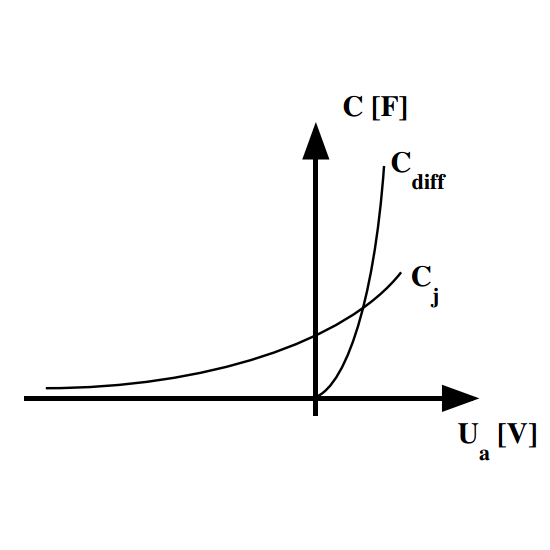
\includegraphics[scale=0.3]{capp.png}
\caption{The two capacitances that can be seen in a pn-junction}
\label{capp}
\end{figure}

\section{Methods}
\subsection{PN junction UI}
\begin{figure}[H]
	\centering
	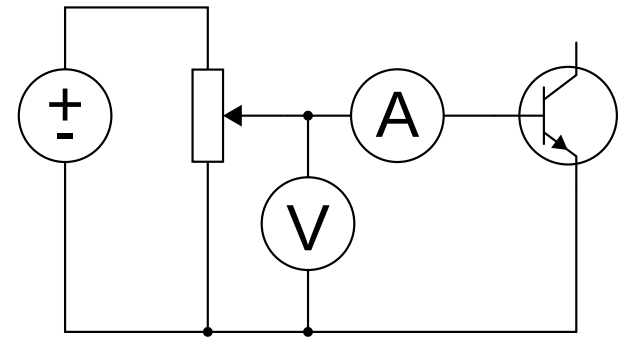
\includegraphics[width=0.3\textwidth]{ui_koppling.png}
	\caption{Circuit used for UI examination.}
	\label{ui_koppling}
\end{figure}
The circuit in figure \ref{ui_koppling} was used to measure the UI characteristics of the PN junction. The voltage was measured over a single junction in the transistor using a voltage meter and the current through it was measured on the base in the transistor as you can see in the figure.

The potentiometer shown in figure \ref{ui_koppling} was used to controll the voltage over the junction. By sweeping the voltage from 0 to 750mV and read off the values on the ampere meter and the voltage meter a graph could be ploted.

\subsection{PN junction capacitance}
To measure the capacitance in a PN junction a capacitance meter was used. By connecting a voltage source to the meter, the voltage over the capacitance could be controlled. By sweeping the voltage from 0 to 1 volts and reading values of the meter every 0.2 volts, the charateristics of the capacitance in forward voltage mode could be ploted. To meassure the characteristics in the reverse voltage mode, the voltage source was switched turned around so the voltage over the pn junction was reversed. In the reverse mode, the voltage was swept from 0 to -2 volts and values where read off every 0.2V. The result was ploted using matlab.

\subsection{NPN transistor}
The examination of the NPN transistor was a little bit more challenging than for the PN junction. The following circuit was used.

\begin{figure}[H]
	\centering
	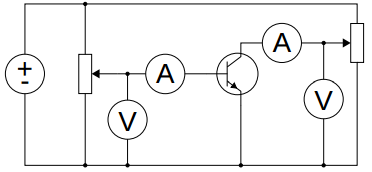
\includegraphics[width=0.3\textwidth]{npn_circuit.png}
	\caption{Circuit used for examination of the NPN transistor}
	\label{npn_koppling}
\end{figure}
To get both graphs showin the result, two sweeps had to be done. First a sweep where the base voltage was kept constant at 0,6V (using the potentiometers) and the collector voltage was swept from 0V and 0.25V, the values was read off every 25mV.

For the second sweep the collector voltage was keept constant at a value of 0.5V and the base voltage was swept between 0V and 0.7. For this examination the values where read off every 50mV.

The result from the sweeps were ploted using matlab. Both the current to $U_{CE}$ and current to $U_{BE}$ were ploted.

\section{Result}
\subsection{PN junction UI}
The following graph was plotted for the PN junction U-I characteristics. See the measured data in the appendix together with the matlab-code. 
\begin{figure}[H]
	\centering
	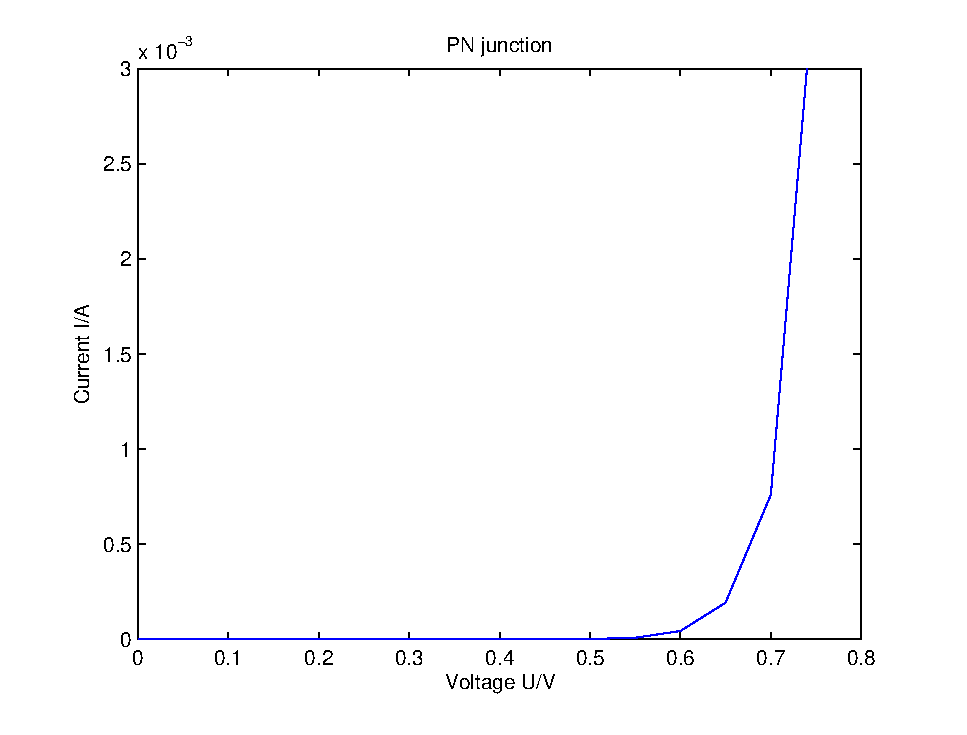
\includegraphics[width=0.7\textwidth]{pn_ui.eps}
	\caption{U-I characterstics for the PN junction.}
	\label{pn_ui}
\end{figure}

\subsection{PN junction capacitance}
The following graph was plotted using the measured data in the appendix for the capacitance in the PN junction. See appendix for values and matlab-code. 
\begin{figure}[H]
	\centering
	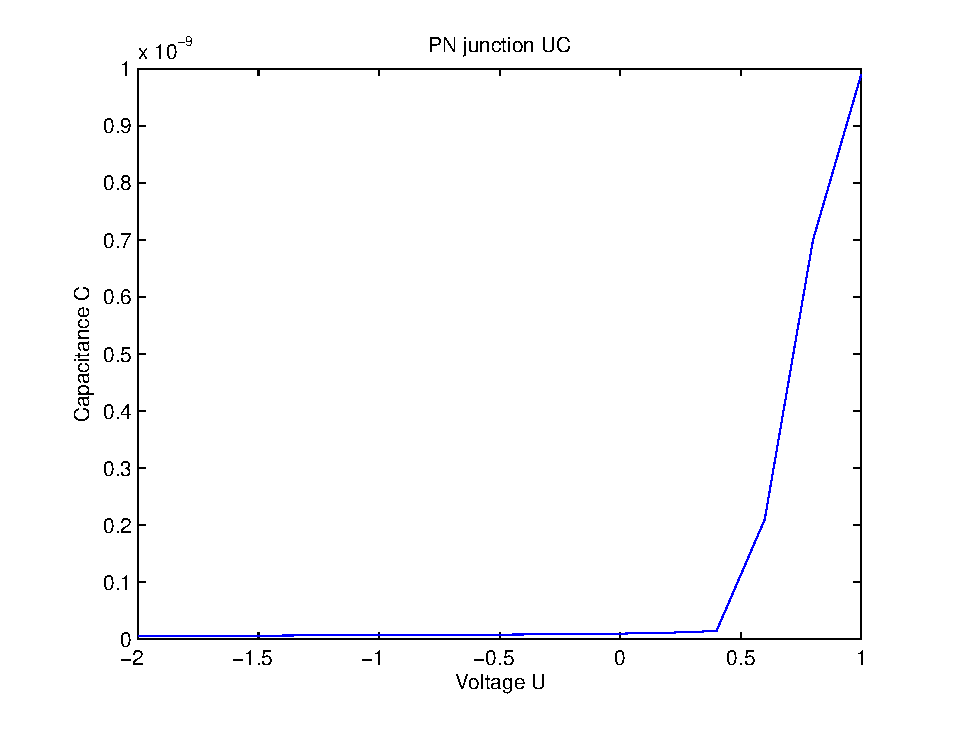
\includegraphics[width=0.7\textwidth]{pn_cap.eps}
	\caption{C-U characterstics for the PN junction.}	
	\label{pn_cap}
\end{figure}
\begin{figure}[H]
	\centering
	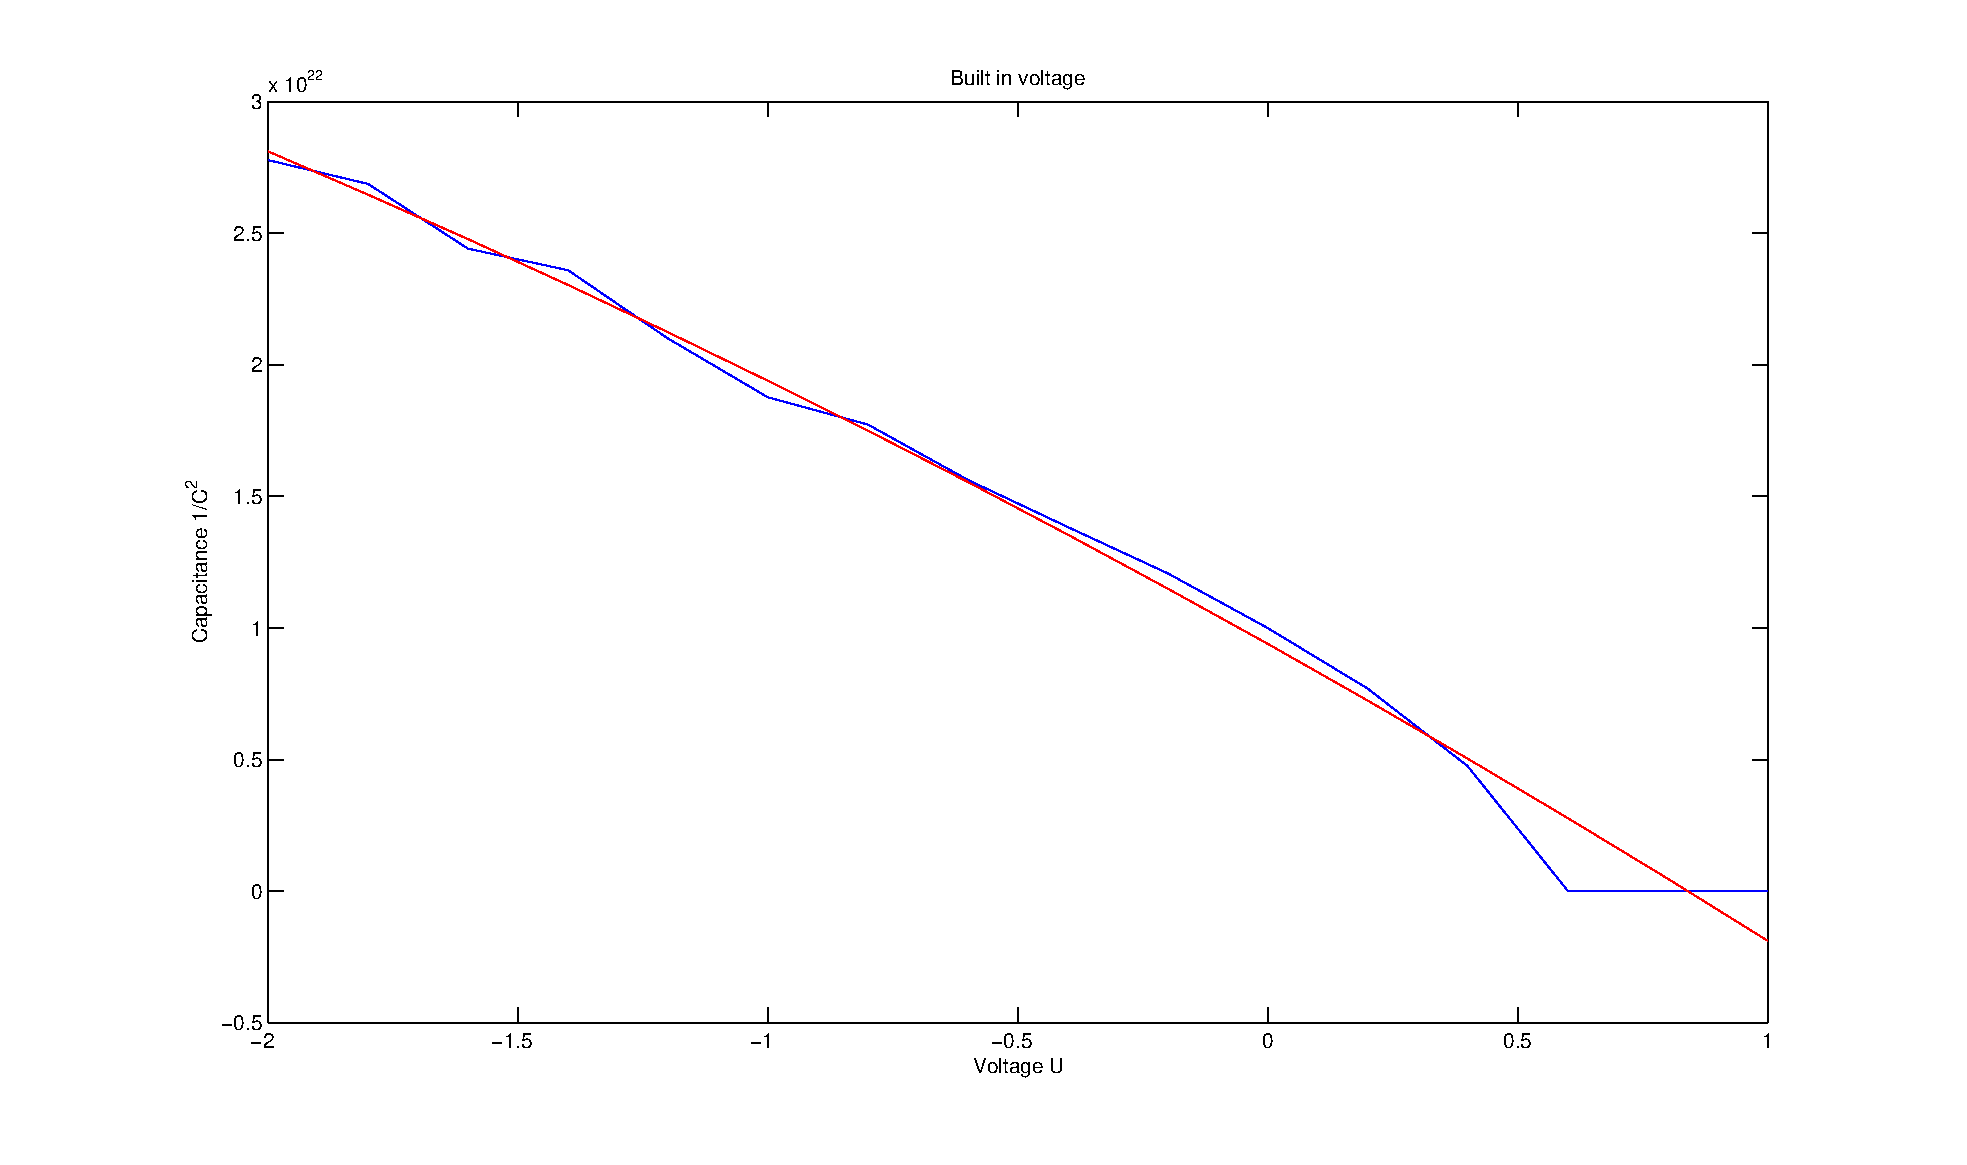
\includegraphics[width=0.7\textwidth]{built_in_v.eps}
	\caption{Plot to get the built in voltage. The red line is a linear aproximation of the blue.}
	\label{pn_cap_built_in_v}
\end{figure}

The built in voltage was calculated to $0,9V$.

\subsection{NPN transistor}
The following graphs were plotted for the current in the npn transistor. The early voltage was calculated to 34V using matlab. See the appendix for values and matlab-code.
\begin{figure}[H]
	\centering
	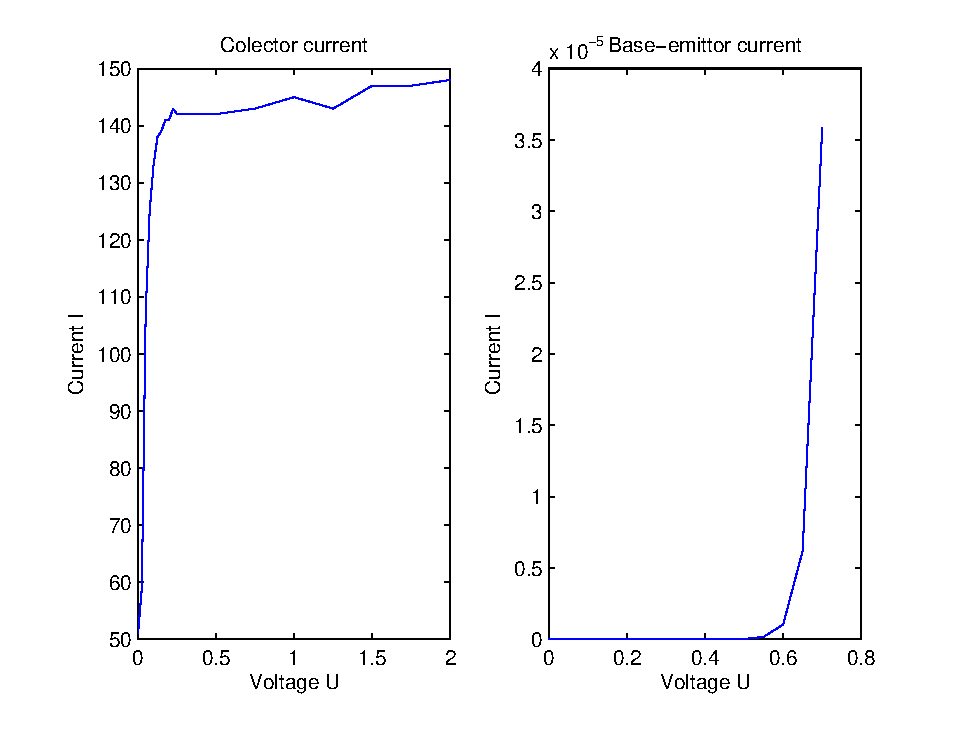
\includegraphics[width=0.85\textwidth]{npn.eps}
	\caption{Voltage to current characteristics for the NPN transistor. The collector current to the left and the base-emittor current to the right.}	
	\label{npn}
\end{figure}

\newpage
\section{Analysis of the result}
\subsection{PN junction UI}
In figure \ref{pn_ui} the current to voltage ratio is plotted from the measured values. Since this is a PN junction it is expected to behave like a normal diode. In the graph it is clear that the current through the pn junction is zero until it the voltage over the junction reches about 0.7V. This value of the forward voltage is expected and is about the same for all pn junctions.

\subsection{PN junction capacitance}
The capacitance in a transistor consists of both a junction capacitance and a difusion capacitance. If you apply a negative voltage, only the junction capacitance will be seen. This junction capacitance is very small for very negative voltages but grows bigger for positive values, see figure \ref{capp}. This can be observed in the result in figure \ref{pn_cap}. Here we can see a very small capacitance for negative voltages.

For positive voltages we have both the junction capacitance and the diferential capacitance. The diferential capacitance is very large and grows quickly for positive voltages. This can clearly be observed in figure \ref{pn_cap} as it grows very much and fast for positive values.

To retrive the built in voltage for the PN-junction figure \ref{pn_cap_built_in_v} was ploted. In the graph, the red line is a linear aproximation to the meassured data. The built in voltage can be found where this line crosses the x-axis wich was retrieved by using the approximated polynomial expression $u$. $ u = ax + b = 0 \rightarrow x = -\frac{b}{a} = \frac{9,0128}{9,9970} = 0,9V$.

\subsection{NPN transistor}
As you can see to the left in figure \ref{npn} an increasing voltage from zero to about 0.25 volts results in a substantially increase in the collector current. The current does'nt increase to infinity and beyond though. The current that flows through the transistor is dependent on the current that the powersource can deliver. The steep increase in current stops since there are no more electrons that can diffuse from the emittor through the base to the collector in the transistor.

To calculate the early voltage a linear function was aproximated to the eleven largest values that were measured. To find the aproximation function $p(U) = ax + b$ polyfit was used in matlab (see appendix). Using the function and calculating $p(U) = 0 => x = \frac{b}{a}$ the earlyvoltage was found to be $\frac{139,9}{4,1} \approx 34V$.

The right graph in figure \ref{npn} shows the current that flows from the base to the emittor. Since this is a pn-junction it was expected that the current to voltage graph would look like a diodes graph, which it does. The forward voltage for the pn-junction is shown in the graph to be about 0.6-0.7 V which is normal vlue expected for a diode.

\newpage
\appendix
\section{Matlab code}
\subsection{PN junction UI}
\lstinputlisting{pn_current.m}
\subsection{PN junction capacitance}
\lstinputlisting{pn_cap.m}
\subsection{NPN current}
\lstinputlisting{npn.m}

\newpage
\section{Reference}
Komponentfysik  7 upplagan 2011 - Anders Gustafsson

Komponentfysik - Den bipolära transistorn - Martin Berg och Elvedin Elvedin Memišević
\end{document}
